%------------------------------------------------------------------------------
% Author(s):
% Varaun Ramgoolie
%
% Copyright:
%  Copyright (C) 2020 Brad Bachu, Arjun Mohammed, Varaun Ramgoolie, Nicholas Sammy
%
%  This file is part of Applied-Mathematics-Unit2 and is distributed under the
%  terms of the MIT License. See the LICENSE file for details.
%
%  Description:
%     Year: 2010
%     Module: 3
%     Question: 6
%------------------------------------------------------------------------------

%------------------------------------------------------------------------------
% 6 a
%------------------------------------------------------------------------------

\begin{subquestions}
	
\subquestion
We are given a weight which is attached to a fixed point by an inelastic string.

\begin{subsubquestions}
	
\subsubquestion

\textbf{\textit{Sketch and Translate:}} \\ \\
\begin{figure}[H]
	\begin{center}
		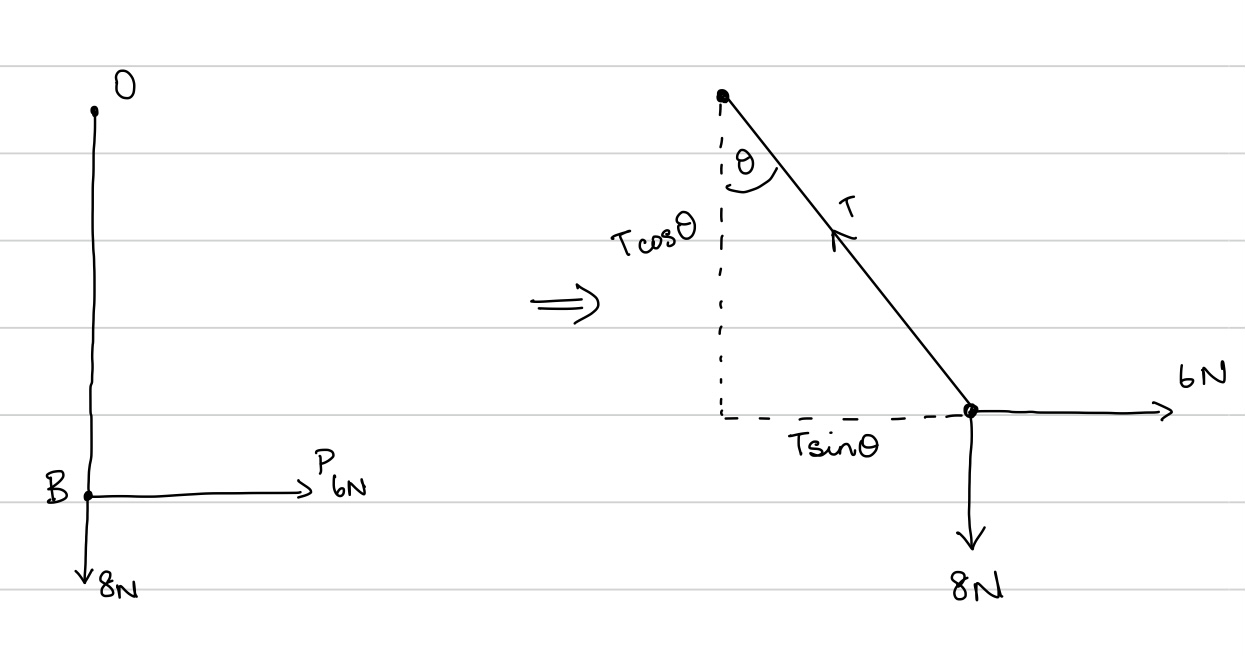
\includegraphics[scale=0.25]{../2010/figures/2010q6-1}
		\caption{\label{2010:q6:Sketch1} Weight attached to at $O$.}
	\end{center}
\end{figure}
We are given that the string is inelastic, which means that the string cannot change size. As we are given forces acting on the weight at $B$, we should begin thinking about how we can use the relationship between these forces to solve for the tension.




\textbf{\textit{Simplify and Diagram:}} \\ \\
\begin{figure}[H]
	\begin{center}
		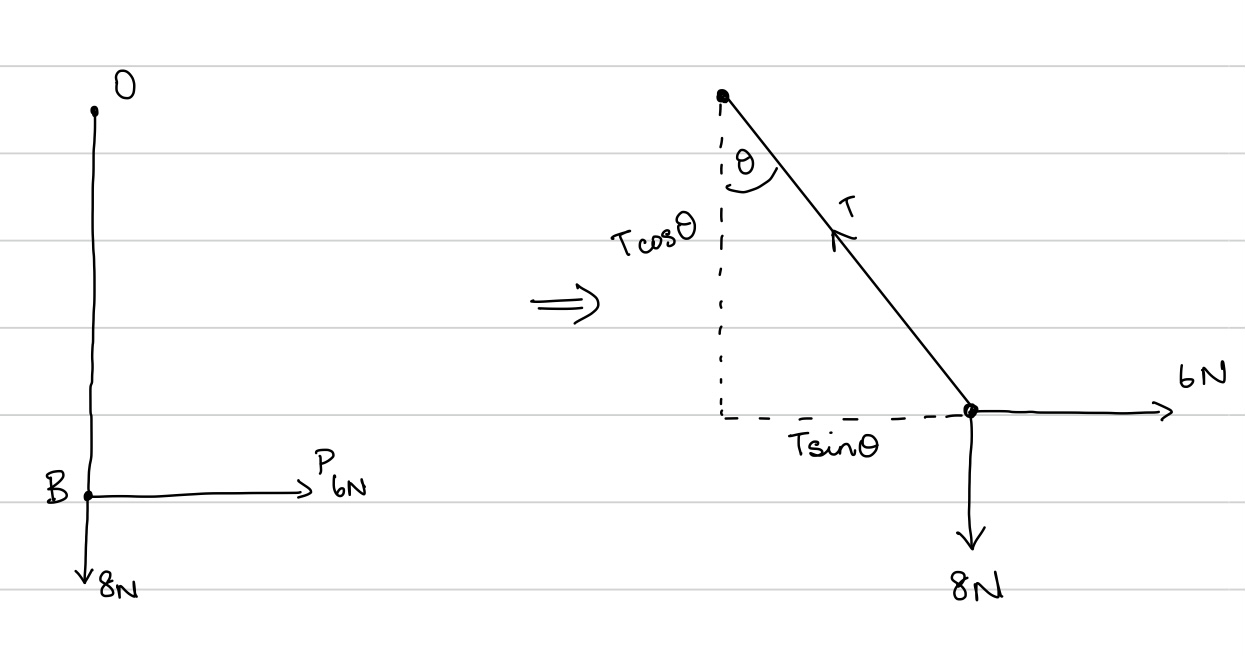
\includegraphics[scale=0.25]{../2010/figures/2010q6-1}
		\caption{\label{2010:q6:DIagram1} Weight attached to at $O$.}
	\end{center}
\end{figure}
We will assume that the string is also massless, which means that the tension at every point along the string is the same. We will define the following:
\begin{itemize}
	\item $\vec{P}$ is the horizontal pull which acts at $B$,
	\item $\vec{W}$ is the weight of the mass,
	\item $\vec{T}$ is the tension is the string acting from $B$ to $O$.
\end{itemize}
As we are given that the system is in equilibrium, we can use Newton's Second Law and resolve the forces to find the magnitude of the tension. 




\textbf{\textit{Represent Mathematically:}} \\ \\
We will first resolve our forces as,
\begin{align}
	\vec{P} & = |P|\xhat \nn \\
	        & = 6\xhat \,. \\
	\vec{W} & = -|W|\yhat \nn \\
	        & = -8\yhat \,. \\ 
	\vec{T} & = -|T|\sin(\theta)\xhat + |T|\cos(\theta)\yhat \,.
\end{align}
where $\theta$ is the angle that OB makes with the normal at $O$.

From Newton's Second Law, in equilibrium, we know that,
\begin{align}
	\sum \vec{F} & = 0 \nn \\
	\implies \sum F_x & = 0 \label{2010:q6:ForceX} \\
	& \text{and} \nn \\
	\implies \sum F_y & = 0 \label{2010:q6:ForceY} \,.
\end{align}
where $F_x$ and $F_y$ are the components of the forces in the $x$ and $y$ directions.



\textbf{\textit{Solve and Evaluate:}} \\ \\
From \req{2010:q6:ForceX}, we get that,
\begin{align}
	\sum F_x & = 0 \nn \\
	6 -|T|\sin(\theta) & = 0 \nn \\
	\implies |T|\sin(\theta) & = 6 \label{2010:q6:TensEqn1} \,.
\end{align}

From \req{2010:q6:ForceY}, we get that,
\begin{align}
	\sum F_y & = 0 \nn \\
	-8 +|T|\cos(\theta) & = 0 \nn \\
	\implies |T|\cos(\theta) & = 8 \,.
\end{align}

Thus, we get that,
\begin{align}
	(|T|\sin(\theta))^2 + (|T|\cos(\theta))^2 & = 6^2 + 8^2 \nn \\
	|T|^2 \left(\sin^2(\theta)+\cos^2(\theta)\right) & = 100 \nn \\
	\implies T & = 10N \,.
\end{align}
	
%------------------------------------------------------------------------------

\subsubquestion

\textbf{\textit{Solve and Evaluate:}} \\ \\
Substituting our value from (a)(i) into \req{2010:q6:TensEqn1}, we get that,
\begin{align}
	|T|\sin(\theta) & = 6 \nn \\
	\implies \theta & = \arcsin(\frac{6}{10}) \nn \\
	                & = 36.87^o \,.
\end{align}
	
\end{subsubquestions}

%------------------------------------------------------------------------------
% 6 b
%------------------------------------------------------------------------------

\subquestion

\begin{subsubquestions}
	
\subsubquestion

\textbf{\textit{Simplify and Diagram:}} \\ \\
\begin{figure}[H]
	\begin{center}
		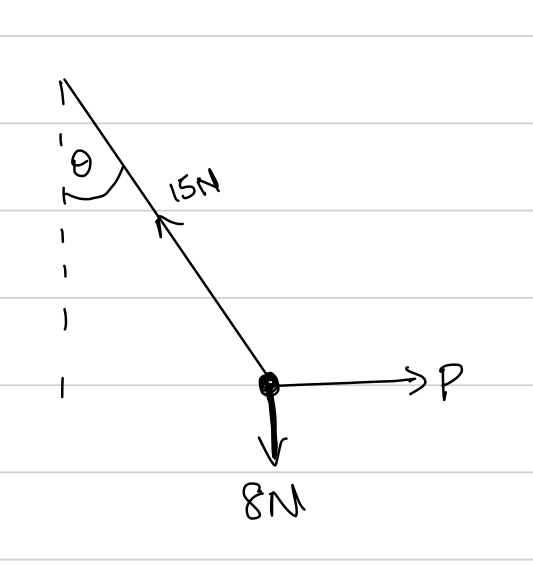
\includegraphics[scale=0.25]{../2010/figures/2010q6-2}
		\caption{\label{2010:q6:Diagram2} String at breaking point.}
	\end{center}
\end{figure}
This question is quite similar to (a) and so, the method used to solve will not be very different. Again, we will use Newton's Second Law and resolve the forces on the mass. We will use the same notation as defined in (a)(i) and we will assume that the system is in equilibrium.





\textbf{\textit{Represent Mathematically:}} \\ \\ 
We will first resolve our forces as,
\begin{align}
	\vec{P} & = |P|\xhat \,. \\ 
	\vec{W} & = -|W|\yhat \nn \\
			& = -8\yhat \,. \\ 
	\vec{T} & = -|T|\sin(\alpha)\xhat + |T|\cos(\alpha)\yhat \nn \\
	        & = -15\sin(\alpha)\xhat + 15\cos(\alpha)\yhat
\end{align}
where $\alpha$ is the angle that OB makes with the normal at $O$.
	
From Newton's Second Law, in equilibrium, we know that,
\begin{align}
	\sum \vec{F} & = 0 \nn \\
	\implies \sum F_x & = 0 \label{2010:q6:ForceX2} \\
	& \text{and} \nn \\
	\implies \sum F_y & = 0 \label{2010:q6:ForceY2} \,.
\end{align}
where $F_x$ and $F_y$ are the components of the forces in the $x$ and $y$ directions.
	



\textbf{\textit{Solve and Evaluate:}} \\ \\
By using \req{2010:q6:ForceY2}, we get that,
\begin{align}
	-8 + 15\cos(\alpha) & = 0 \nn \\
	\implies \alpha & = \arccos\left(\frac{8}{15}\right) \nn \\
	                & = 57.77^o \,. 
\end{align}

%------------------------------------------------------------------------------

\subsubquestion

\textbf{\textit{Solve and Evaluate:}} \\ \\
Substituting our value from (b)(i) into \req{2010:q6:ForceX2}, we get that,
\begin{align}
	\sum F_x & = 0 \nn \\
	|P| - 15\sin(\alpha) & = 0 \nn \\ 
	\implies |P| & = 15\left(\sqrt{1-\cos^2(\alpha)} \right) \nn \\
	             & = 15\left(\sqrt{1-\left(\frac{8}{15}\right)^2} \right) \nn \\
	             & = \sqrt{15^2-8^2} \nn \\
	             & = \sqrt{161} \,.
\end{align}
	
\end{subsubquestions}

%------------------------------------------------------------------------------
% 6 c
%------------------------------------------------------------------------------

\subquestion
We are now given a particle which is influenced by 3 forces.
\begin{subsubquestions}

\subsubquestion

\textbf{\textit{Sketch and Translate:}} \\ \\
\begin{figure}[H]
	\begin{center}
		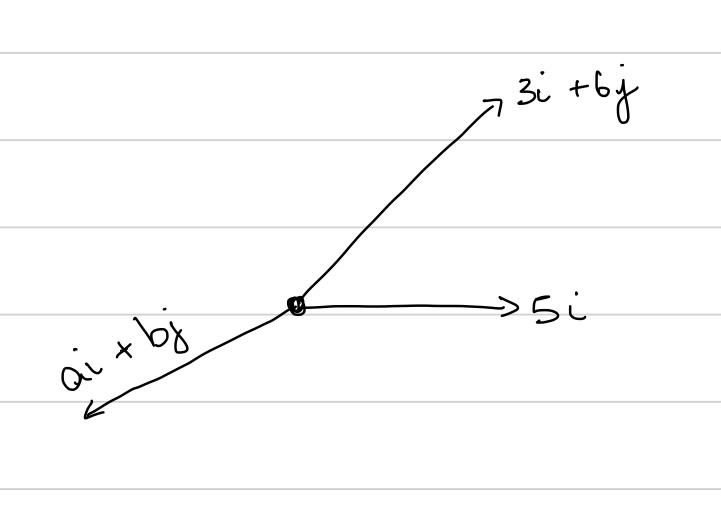
\includegraphics[scale=0.25]{../2010/figures/2010q6-3}
		\caption{\label{2010:q6:Sketch3} Particle impacted by the 3 forces.}
	\end{center}
\end{figure}
As the particle is in equilibrium, we get that there is no resultant force on the body. We should think about how we can express this system in order to solve the problem.




\textbf{\textit{Simplify and Diagram:}} \\ \\
\begin{figure}[H]
	\begin{center}
		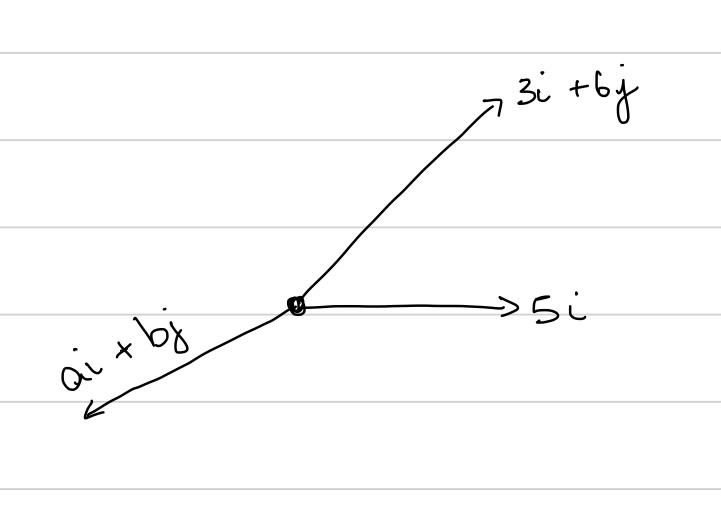
\includegraphics[scale=0.25]{../2010/figures/2010q6-3}
		\caption{\label{2010:q6:Diagram3} Particle impacted by the 3 forces.}
	\end{center}
\end{figure}
We will define the forces as,
\begin{itemize}
	\item $\vec{Q}=5\ihat$,
	\item $\vec{R}=3\ihat+6\jhat$,
	\item $\vec{S}=a\ihat+b\jhat$.
\end{itemize}
As they are already expressed in terms of unit vectors along the horizontal and vertical directions, we can directly apply Newton's Second Law to the system in equilibrium.




\textbf{\textit{Represent Mathematically:}} \\ \\
From Newton's Second Law, in equilibrium, we know that,
\begin{align}
	\sum \vec{F} & = 0 \nn \\
	\implies \sum F_i & = 0 \label{2010:q6:ForceI} \\
	& \text{and} \nn \\
	\implies \sum F_j & = 0 \label{2010:q6:ForceJ} \,.
\end{align}
where $F_i$ and $F_j$ are the components of the forces in the horizontal and vertical directions respectively.




\textbf{\textit{Solve and Evaluate:}} \\ \\
From \req{2010:q6:ForceI}, we get that,
\begin{align}
	5+3+a & = 0 \nn \\
	\implies a & = -8 \,.
\end{align}

From \req{2010:q6:ForceJ}, we get that,
\begin{align}
	6+b & = 0 \nn \\
	\implies b & = -6 \,.
\end{align}

We now have that,
\begin{equation}
	\vec{S} = -8\ihat -6\jhat \,.
\end{equation}

We can then find that,
\begin{align}
	|\vec{S}| & = \sqrt{(-6)^2+(-8)^2} \nn \\
	          & = 10N
\end{align}

%------------------------------------------------------------------------------

\subsubquestion

\textbf{\textit{Simplify and Diagram:}} \\ \\
\begin{figure}[H]
	\begin{center}
		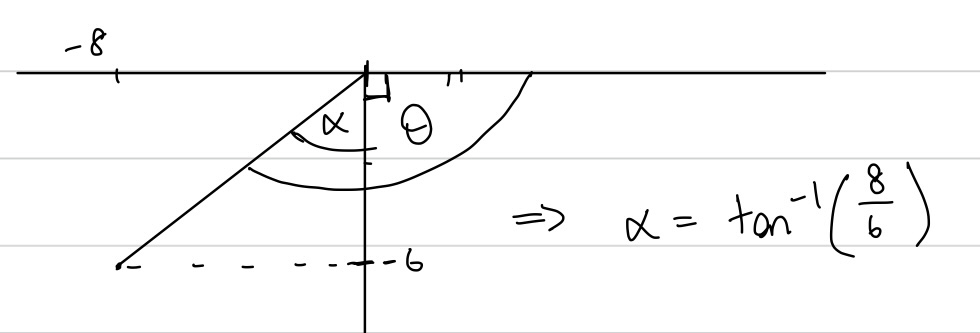
\includegraphics[scale=0.25]{../2010/figures/2010q6-4}
		\caption{\label{2010:q6:Diagram4} Angle of $\vec{S}$.}
	\end{center}
\end{figure}
Using our knowledge of trigonometry, we can easily solve for the angle that $\vec{S}$ makes with the vertical, given as $\beta$. We can then find the angle that $\vec{S}$ makes with $Ox$.




\textbf{\textit{Represent Mathematically:}} \\ \\
We get that,
\begin{equation}
	\tan(\beta) = \frac{-8}{-6} \,.
\end{equation}




\textbf{\textit{Solve and Evaluate:}} \\ \\
We can now find that,
\begin{align}
	\beta & = \arctan\left(\frac{-8}{-6}\right) \nn \\
	      & = 53.13^o \,.
\end{align}

Thus, we get that $\vec{S}$ makes a clockwise angle of $(90+53.13)^o$ from $Ox$.\footnote{This is equivalent to making an anticlockwise angle of $(180+36.87)^o$ from $Ox$.}



\end{subsubquestions}




\end{subquestions}